\documentclass[]{politex}
% ========== Opções ==========
% pnumromarab - Numeração de páginas usando algarismos romanos na parte pré-textual e arábicos na parte textual
% abnttoc - Forçar paginação no sumário conforme ABNT (inclui "p." na frente das páginas)
% normalnum - Numeração contínua de figuras e tabelas 
%	(caso contrário, a numeração é reiniciada a cada capítulo)
% draftprint - Ajusta as margens para impressão de rascunhos
%	(reduz a margem interna)
% twosideprint - Ajusta as margens para impressão frente e verso
% capsec - Forçar letras maiúsculas no título das seções
% espacosimples - Documento usando espaçamento simples
% espacoduplo - Documento usando espaçamento duplo
%	(o padrão é usar espaçamento 1.5)
% times - Tenta usar a fonte Times New Roman para o corpo do texto
% noindentfirst - Não indenta o primeiro parágrafo dos capítulos/seções


% ========== Packages ==========
\usepackage[utf8]{inputenc}
\usepackage{amsmath,amsthm,amsfonts,amssymb}
\usepackage{graphicx,cite,enumerate}


% ========== Language options ==========
\usepackage[brazil,english]{babel}
%\usepackage[english]{babel}


% ========== ABNT (requer ABNTeX 2) ==========
%	http://www.ctan.org/tex-archive/macros/latex/contrib/abntex2
\usepackage[num]{abntex2cite}

% Forçar o abntex2 a usar [ ] nas referências ao invés de ( )
%\citebrackets{[}{]}


% ========== Lorem ipsum ==========
\usepackage{blindtext}



% ========== Opções do documento ==========
% Título
\titulo{Formicarium: Ambiente de desenvolvimento em tempo real para microsserviços}

% Autor
\autor{Leonardo C. S. Iacovini\\
		Luiz G. Santos\\
		Rafael L. D. R. Santos\\
		Rafael R. Correia}

% Para múltiplos autores (TCC)
%\autor{Nome Sobrenome\\%
%		Nome Sobrenome\\%
%		Nome Sobrenome}

% Orientador / Coorientador
\orientador{Jorge Risco Becerra}
\coorientador{Rafael de França Ferreira}

% Tipo de documento
\tcc{Engenharia de Computação}
%\dissertacao{Engenharia Elétrica}
%\teseDOC{Engenharia Elétrica}
%\teseLD
%\memorialLD

% Departamento e área de concentração
\departamento{PCS}
\areaConcentracao{Engenharia de Software}

% Local
\local{São Paulo}

% Ano
\data{2018}




\begin{document}
% ========== Capa e folhas de rosto ==========
\capa
% \falsafolhaderosto
\folhaderosto


% ========== Folha de assinaturas (opcional) ==========
%\begin{folhadeaprovacao}
%	\assinatura{Prof.\ X}
%	\assinatura{Prof.\ Y}
%	\assinatura{Prof.\ Z}
%\end{folhadeaprovacao}


% ========== Ficha catalográfica ==========
% Fazer solicitação no site:
%	http://www.poli.usp.br/en/bibliotecas/servicos/catalogacao-na-publicacao.html


% ========== Dedicatória (opcional) ==========
%\dedicatoria{Dedicatória}


% ========== Agradecimentos ==========
\begin{agradecimentos}

Valeu Risco

\end{agradecimentos}


% ========== Epígrafe (opcional) ==========
%\epigrafe{%
%	\emph{``Epígrafe''}
%	\begin{flushright}
%		-{}- Autor
%	\end{flushright}
%}


% ========== Resumo ==========
\begin{resumo}
	Em uma arquitetura distribuída de microsserviços, é comum enfrentar problemas relacionados à produtividade enquanto o software é desenvolvido. Uma das causas deste problema é a necessidade de se executar diversos micro serviços ao mesmo tempo para iterar, testar e validar algum fluxo de negócio. Estes processos computacionais demandam uma quantidade de recursos (processamento e memória) que nem sempre estão disponíveis na máquina do desenvolvedor.
	
	Um outro problema comum é a dificuldade de se entender e depurar fluxos complexos de negócio que envolvam comunicação entre diversos micro serviços através de diferentes protocolos de troca de mensagens.
	
	Foi neste contexto que surgiu a parceria entre a Poli e o Nubank para o desenvolvimento de um projeto que tentasse mitigar os problemas acima descritos.
	
	O Nubank é uma fintech brasileira que conta com mais de 200 engenheiros, trabalhando diariamente em mais de 200 micro serviços para atender os mais de 5 milhões de clientes ativos em seus diversos produtos. A empresa é referência nacional e mundial em tecnologia, devido a sua arquitetura de software moderna, baseada em micro serviços. Porém, as implicações negativas deste modelo já estão se manifestando na empresa há algum tempo, prejudicando a produtividade das equipes.
	
	O projeto foi co-orientado por um dos engenheiros mais prestigiados do Nubank, que está presente na empresa desde praticamente o seu nascimento, sendo responsável por importantes decisões arquiteturais e por ter participado da construção da fundação de toda a tecnologia da empresa.
	
	Através do intenso uso de computação em nuvem, orquestração de Containers Docker, conceitos de Distributed Tracing e técnicas para sincronização de file systems, este projeto visa aumentar a produtividade dos engenheiros do Nubank em suas tarefas de desenvolvimento e manutenção dos micro serviços da empresa.
	
	Para o desenho da solução, foi feito um estudo profundo sobre modelos de PaaS, características de micro serviços de modo geral, bem como seu uso no contexto específico do Nubank. 
	
	O resultado foi a construção de um ambiente de desenvolvimento para arquiteturas de larga escala baseada em micro serviços, chamado de Formicarium. O projeto foi implantado em um squad do Nubank nos últimos meses de desenvolvimento do trabalho para que feedbacks pudessem ser colhidos e para que fossem feitos os ajustes necessários.
	
	Com base nos resultados, pode-se concluir que o projeto conseguiu atender os requisitos propostos e mitigar os diversos problemas apresentados. A sua implantação foi bem recebida pelo squad escolhido e sua difusão não é uma tarefa complicada, dado sua fácil utilização e vantagens imediatas. Inclusive, ao longo do projeto foi tomado o cuidado de se extrair os componentes altamente acoplados com características específicas do Nubank, de modo que a implantação da solução até mesmo em outras empresas fosse possível sem muitas modificações.
	
%
% \\[3\baselineskip]
%
\textbf{Palavras-Chave} -- Microsserviço, Docker, Kubernetes, Computação em Nuvem, Distributed Tracing.
\end{resumo}


% ========== Abstract ==========
\begin{abstract}
Abstract...
%
\\[3\baselineskip]
%
\textbf{Keywords} -- Word, Word, Word, Word, Word.
\end{abstract}


% ========== Listas (opcional) ==========
%\listadefiguras
%\listadetabelas

% ========== Listas definidas pelo usuário (opcional) ==========
%\begin{pretextualsection}{Lista de símbolos}

%Lista de símbolos...

%\end{pretextualsection}

% ========== Sumário ==========
\sumario



% ========== Elementos textuais ==========

%\part{Introdução}
	
\chapter{Introdução}
	\section{Objetivo}
	\section{Motivação}
	A motivação desse projeto vem de alguns fatores. O primeiro é o interesse e a familiaridade do grupo quanto ao desenvolvimento de microsserviços provenientes da experiência adquirida nos estágios na Nubank, e o reconhecimento dos benefícios e dificuldades essa arquitetura. Outro fator importante é a constatação de que, com o crescimento das aplicações em nuvem computacional, a necessidade e urgência de uma arquitetura distribuída aumenta, e a carência de ferramentas para conter suas dificuldades se torna um problema cada vez mais importante.
	
	Com isso, foi possível a identificação de um problema relativamente complexo de Engenharia de Software que ainda não teve a devida atenção no mercado, e uma oportunidade para aplicação e aprofundamento do nosso conhecimento de processo de desenvolvimento de software. Nós queríamos, então, criar uma proposta de solução para um problema real ainda em discussão.
	\section{Justificativa}
	
	\section{Organização do Trabalho}
	
\chapter{Aspectos Conceituais}
	\section{Docker}
	\subsection{Breve história das tecnologias de contêineres}
	A história dos Contêineres começa em 1979 no Unix L7. Nele foi introduzido a chamada de sistema (system call) chroot capaz de mudar o diretório raiz de um processo e de seus processos filhos para um novo local no filesystem. Este avanço foi o início do conceito de isolamento de processos, pois limitava o acesso de cada processo ao sistema de arquivos. 

	Em 2000, surgiu o FreeBSD Jail, que permite a administradores particionar um sistema FreeBSD em vários sistemas menores isolados e independentes, chamados de “Jails”. O sistema é similar ao chroot, mas incluiu recursos de isolamento adicionais em diversos aspectos do sistema operacional, como por exemplo a atribuição de um endereço de IP diferente para cada Jail. [1]

	Em 2001, foi lançado o Linux VServer que, assim como o FreeBSD Jail, também é um mecanismo de Jail que pode particionar recursos (sistema de arquivos, endereços de rede, memória) em um sistema computacional. Isso é realizado por meio de níveis de isolamento do kernel. Cada partição é chamada Security Context e o sistema virtualizado dentro dele é chamado de Virtual Private Server [2]

	Em 2004, foi lançado o Solaris Zones para sistemas x86 e SPARC. Cada Zone age como um servidor virtual completamente isolado dentro de uma única instância Existem dois tipos de Solaris Zones: zonas globais (Global Zones) e não-globais (Non-Global Zones). A zona global é o ambiente de SO tradicional e é a área onde o SO Solaris está instalado. Todas as operações do sistema, como instalações, inicializações e desligamentos são feitas na zona global. As zonas não-globais, comumente chamadas somente de zonas, tem seus recurso e limites definidos pela zona global a que pertencem  [3]

	Em 2005 a empresa Virtuozzo lançou o OpenVZ, que utiliza o kernel do Linux para fornecer virtualização, isolamento, gerenciamento de recursos e checkpointing. Cada contêiner OpenVZ possui um sistema de arquivos isolado, usuários e grupos de usuários, uma árvore de processos, rede, dispositivos e comunicação entre processos. Uma desvantagem da solução é que seu funcionamento depende da aplicação de um patch no kernel do Linux. [4]

	Em 2006 engenheiros da Google desenvolveram o Process Containers, projetado para limitar, contabilizar e isolar o uso de recursos computacionais (CPU, memória, I/O do disco, rede) de uma coleção de processos. Um ano depois o projeto foi renomeado para Control Groups (cgroups) e foi adicionado ao kernel do Linux na versão 2.6.24.

	Em 2008 surgiu o LXC (LinuX Containers), que foi a primeira e mais completa implementação de um gerenciador de contêineres Linux. Foi implementado utilizando cgroups e Linux namespaces e funciona no kernel do Linux sem a necessidade da aplicação de patches.
	Em 2011 a empresa CloudFoundry iniciou o projeto Warden, que usava LXC em suas primeiras implementações, porém depois foi substituído por soluções próprias da empresa. Warden roda em formato daemon e pode isolar ambientes em qualquer sistema operacional. Além disso, provê uma API para o gerenciamento de cgroups, namespaces, ciclo de vida dos processos e dos containers em diversos hosts através de um modelo cliente-servidor.

	Finalmente, em 2013, surgiu o Docker. Neste momento Contêineres cresceram muito em popularidade, juntamente com o Docker em si.
	Assim como o Warden, o Docker utilizou LXC em seus primeiros estágios mas logo trocou por uma solução própria para gerenciamento de contêineres: o libcontainer.
	O Docker se destacou de seus concorrentes por oferecer um ecossistema completo para o gerenciamento de Containers, que será detalhado a seguir.
	
	\subsection{Contêineres vs Máquinas virtuais}
	
	A Virtualização é a tecnologia que permite a criação de diferentes ambientes computacionais, chamados de virtuais por simular a interface que é esperada por um sistema operacional.
	
	Um dos principais componentes da arquitetura é o Hypervisor. Ele gerencia a distribuição dos recursos computacionais na máquina física (armazenamento, processamento e memória) entre as várias Máquinas Virtuais, além de fornecer um isolamento entre elas. Ele é um componente que fica entre o hardware e a máquina virtual e é necessário para o processo de virtualização.
	Entre os maiores provedores de máquinas virtuais no mercado, pode-se citar VMWare vSphere, VirtualBox, Xen, Hyper-V e KVM.

	No baixo nível, um container é apenas um conjunto de processos que são isolados do resto do sistema. No caso do Docker, os contêineres compartilham o kernel do sistema operacional hospedeiro e, frequentemente, os binários e bibliotecas também. Todos os componentes compartilhados são read-only. Este compartilhamento de componentes reduzem a necessidade de se replicar código do sistema operacional, e isso significa que um único servidor pode executar múltiplos contêineres com uma única instalação do sistema operacional.

	Diferentemente, uma máquina virtual é constituída do espaço de usuário juntamente com o espaço do kernel de um sistema operacional e o hardware é virtualizado. Cada máquina virtual tem um sistema operacional e suas aplicações e elas compartilham entre si o hardware do computador hospedeiro.

	Ambas as tecnologias provém ambientes isolados para execução de aplicações e podem ser utilizadas para empacotar e distribuir software.

	Dado o menor número de camadas entre a aplicação e o hardware,  os contêineres tendem a ser mais leves e mais rápidos, tornando-os mais práticos para os ciclos de desenvolvimento e implantação de serviços. Comparativamente, o tempo de inicialização de uma VM é muito maior do que a de um Contêiner equivalente, além de o espaço ocupado em disco ser uma ordem de magnitude maior.
	
	\begin{figure}[htb]
		\caption{\label{fig_circulo}Diferenças entre VMs e Contêiners}
		\begin{center}
		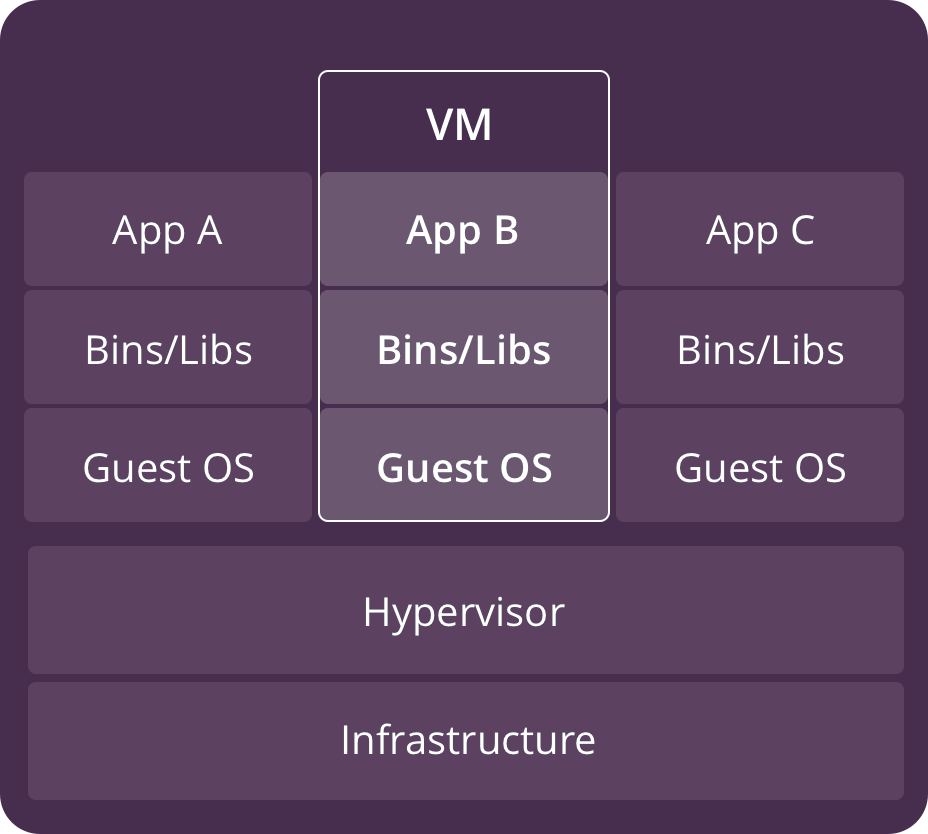
\includegraphics[scale=0.20]{vms.png}
		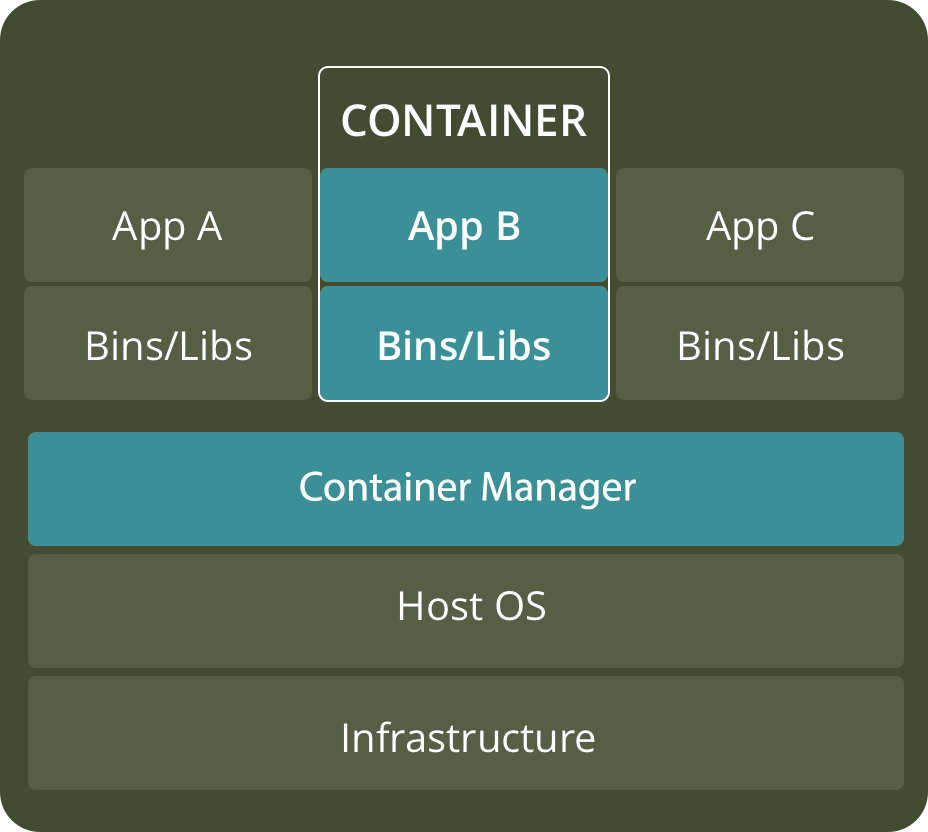
\includegraphics[scale=0.20]{containers.png}
		\end{center}
		% \legend{Fonte: os autores} ABNT HELP
		% \caption{Fonte: https://www.backblaze.com/blog/vm-vs-containers/}
	\end{figure}
	
	Ambos têm vantagens e desvantagens, e a decisão entre um outro varia dependendo dos casos de uso específicos, mas pode-se utilizar as seguintes regras como um ponto de partida:
	
	VMs são melhores para executar aplicações que necessitam de todos os recursos e funcionalidades do sistema operacional ou quando há uma variedade de sistemas operacionais para se gerenciar.
	
	Contêineres são uma escolha melhor quando a maior prioridade é maximizar o número de aplicações sendo executadas em um número mínimo de servidores.
	
	\section{Kubernetes}
	Kubernetes é um projeto de código aberto da Google, que possui mais de 1800 contribuintes e ganha cada vez mais atenção no mundo de operação e desenvolvimento de software. 
	O Google, dado a escala de sua operação, sofria com problemas com o gerenciamento de muitas máquinas virtuais. 
	Assim, o Google precisou repensar como lidar com esse problema, o que, depois de anos, levou ao gerenciador e escalonador de contêiners chamado Kubernetes.

	Para entender melhor a necessidade de um gerenciador tal como o Kubernetes, é necessário dar um passo atrás e olhar para as vantagens e desvantagens dos contêiners.
	Contêiners são feitos para serem leves, rápidos, mas de duração curta e frágeis.
	Assim, eles trocaram a resiliência de uma máquina virtual pela velocidade e leveza. Isso requer que contêiners rodem em um ambiente onde em caso de falha ou mudança de carga, esse ambiente garanta a substituição desses contêiners e gerencie eventuais mudanças de rede e recursos de memória do cluster.
 
\chapter{Tecnologias Utilizadas}
	

\chapter{Metodologia do Trabalho}
	

\chapter{Especificação de Requisitos do Sistema}
	

\chapter{Projeto e Implementação}
	\section{FileSync}

	Um dos grandes desafios do projeto foi a construção de um sistema para sincronização de arquivos em uma arquitetura distribuída de micro serviços.
	
	O caso de uso principal para esta funcionalidade é permitir que o engenheiro da Nubank pudesse iterar de maneira mais rápida no desenvolvimento de um novo micro serviço ou em modificações de algum existente.
	
	Do ponto de vista da empresa, esta era um dos requisitos mais desejados e que mais agregaria valor ao produto final, dado que é uma ferramenta extremamente poderosa para o engenheiro, garantindo-lhe mais produtividade e liberdade enquanto estivesse desenvolvendo.
	
	Este sistema de sincronização de arquivos precisava atender algumas premissas:
	- Deve se integrar facilmente ao workflow do engenheiro, para haver um incentivo à sua adoção.
	- Segurança: Os arquivos trafegados não devem ser, de maneira alguma, expostos para a internet ou suscetíveis a ataques como Man in the middle, dado que o conteúdo trafegado é extremamente sensível (códigos fonte dos produtos da empresa)
	- Velocidade: Quanto mais rápido for o processo de sincronização, mais dinâmico será o processo, permitindo iterações mais rápidas e, consequentemente, maior produtividade.

	Para entender o problema que o sistema de Filesync se propõe a resolver, é preciso entender o cenário:
	
	Os serviços em que o engenheiro está trabalhando não estão sendo compilados e executados na mesma máquina em que está o código fonte. Na verdade eles estão sendo executados em um container Docker, gerenciado por um cluster Kubernetes, operando em uma infraestrutura provida pela AWS EC2. Para que mudanças no código fonte fossem de fato percebidas pelo desenvolvedor, este precisaria compilar uma nova imagem Docker com o código fonte atualizado, publica-lá em um Container Registry e realizar a implantação desta nova imagem no cluster remoto. Este processo, em um contexto de desenvolvimento, é extremamente ineficiente, o que tornaria o processo pouco dinâmico e não atrativo para o engenheiro.

	Para evitar a geração de uma nova imagem Docker a cada iteração no código fonte, foi desenvolvida uma imagem genérica capaz de compilar e executar qualquer serviço da Nubank em modo de desenvolvimento. Esta imagem foi apelidada de Chamber e uma de suas características é a sua extensibilidade, permitindo que em melhorias futuras sejam desenvolvidas versões para outras linguagens e plataformas (Como por exemplo NodeJS, Ruby, Scala, etc.). Para implantação no Nubank, foi desenvolvida a imagem Chamber-lein, capaz de executar programas escritos em Clojure, principal linguagem utilizada nos micro serviços do Nubank.
	\section{Arquitetura da solução}
		\begin{figure}[htb]
			\caption{\label{fig_arquitetura}Arquitetura da solução}
			\begin{center}
			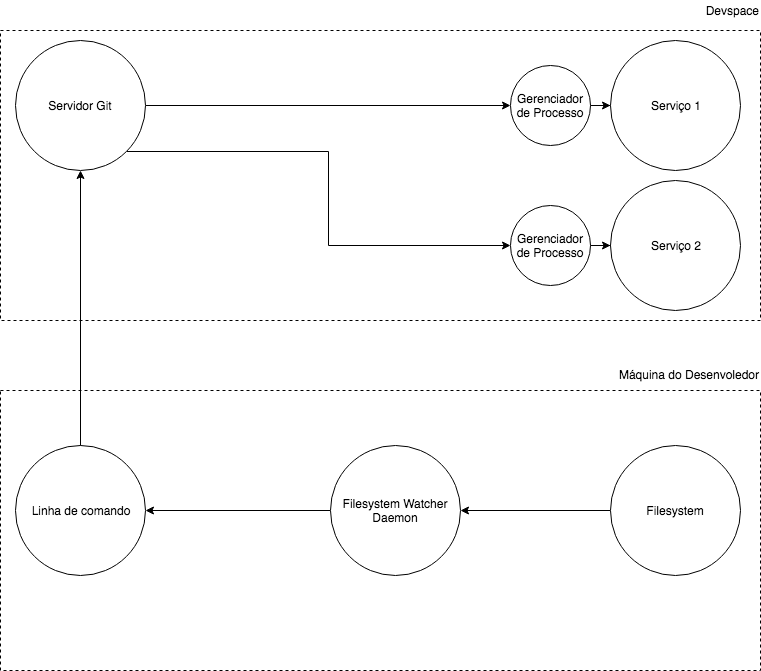
\includegraphics[scale=0.50]{arquitetura-da-solucao.png}
			\end{center}
			% \legend{Fonte: os autores} ABNT HELP
			% \caption{Fonte: própria}
		\end{figure}
	\section{Servidor Git}
	Um dos componentes do sistema de sincronização de arquivos é um servidor web apelidado de Tanajura. O serviço tem como principal responsabilidade ser um hub de repositórios Git.
	
	Nestes repositórios está o código fonte dos serviços que o desenvolvedor está trabalhando no momento e o Git é utilizado como mecanismo de sincronização entre o sistema de arquivos local da máquina do desenvolvedor e o sistema de arquivos do Contêiner em que está sendo executado a aplicação, em um cluster Kubernetes remoto.
	
	O serviço conta com endpoints para gerenciamento de repositórios (operações de criação, remoção e consulta) através de uma interface REST bem como um endpoint que implementa os protocolos de transferência HTTP do Git para realização das operações básicas de Git entre dois peers, como push, pull, fetch.
	
	Os repositórios Git neste serviço têm como característica a efemeridade, ou seja, eles não precisam ser persistidos e só existem para fins de sincronização entre dois file systems, podendo ser sobrescritos e apagados a qualquer momento sem perda de dados.
	
	A escolha do Git para este sistema de sincronização foi devido a algumas de suas características que atendiam os requisitos definidos:
	
	Binário já presente na máquina do desenvolvedor, pois todos trabalham com Git em seu dia-a-dia
	
	Método eficiente para troca de dados, pois os commits são baseados em diff
	
	Troca de dados criptografadas com SSL

	Ao receber um push em algum repositório Git, o Tanajura identifica qual o serviço associado ao repositório e faz uma requisição HTTP para o Soil a fim de obter a URL do Gerenciador de Processo (Stinger) deste serviço.
	
	Uma vez obtida esta URL, o serviço Tanajura faz uma requisição para o Gerenciador avisando-o de que há uma nova versão do código disponível para ser sincronizada.
	
	Este, por sua vez, realiza um pull no repositório remoto para obtenção do código atualizado e, após o recebimento, executa os scripts necessários para recompilação/recarregamento do código.
	
	Esta parte do processo pode ser representada pelo seguinte diagrama de sequência:
		\begin{figure}[htb]
			\caption{\label{fig_arquitetura}Fluxo do Tanajura}
			\begin{center}
			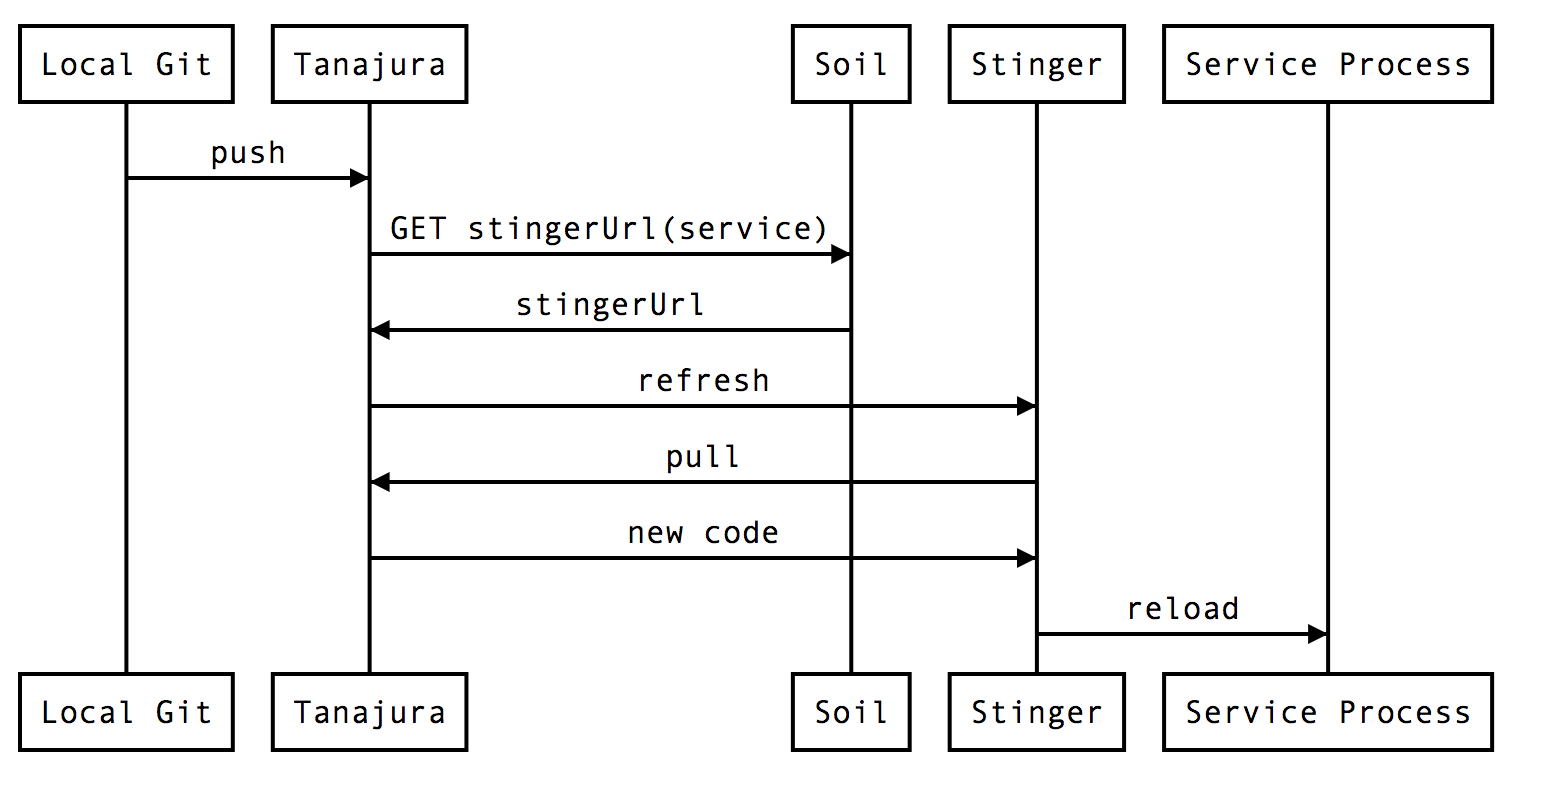
\includegraphics[scale=0.20]{tanajura-flow.png}
			\end{center}
			% \legend{Fonte: os autores} ABNT HELP
			% \caption{Fonte: própria}
		\end{figure}

	Em detalhes, o processo se dá da seguinte maneira:
	
	Quando o desenvolvedor deseja implantar em seu devspace um serviço com capacidades de sincronização, ele digita o seguinte o comando:

	\begin{verbatim}
	fmc service:deploy:local my-service -f ./config-file.json /path/to/service
	\end{verbatim}

	Este comando irá realizar a implantação de um serviço chamado 'my-service', utilizando o arquivo de configuração './config-file.json' a partir da pasta local '/path/to/service'

	\section{Gerenciador de processo (Stinger)}	
	
	Para que fosse possível o método de sincronização de arquivos utilizando Git foi necessário o desenvolvimento de uma aplicação que, através de uma interface HTTP exposta para o Cluster, pudesse fazer pull em um um repositório Git remoto para obtenção do código fonte atualizado e, após o recebimento dos arquivos, fosse possível executar um comando arbitrário para que o processo do serviço pudesse ser recarregado.
	
	Esta aplicação foi apelidada de Stinger e é o binário executado primariamente pela Imagem de Docker Genérica (descrita na próxima sessão).
	
	Os endpoints HTTP disponíveis neste serviço são:

	POST /reset
	
	Ao receber uma requisição neste endpoint, o Stinger termina o processo do serviço em execução através de seu pId (process id) e executa o script de cleanup. Após a garantia de que o processo do serviço foi terminado com êxito, é executa o script de start, que inicia o serviço.
	
	POST /pull
	
	Ao receber uma requisição neste endpoint, o Stinger executa o comando git pull origin master para obter a versão mais recente do código no repositório remoto. É possível, através de parâmetros no corpo da requisição, fazer com que o processo do serviço seja reinicializado logo após o recebimento do código atualizado.

	Quando o Stinger é iniciado, ele verifica a existência do repositório git local e, caso não o encontre, executa o comando git clone [url do repositório] [pasta local] para obter a versão inicial do código. Logo após o recebimento dos arquivos, é feito o processo de inicialização do serviço.

	É possível configurar diversos parâmetros de funcionamento do Stinger através de variáveis de ambiente. Os mais relevantes são:
	
	APP\_PATH
	
	É a o caminho para o diretório local onde o Stinger irá clonar o código do repositório remoto.
	exemplo: /app


	STINGER\_SCRIPTS
	
	Caminho para o diretório local onde o Stinger irá executar os scripts para gerenciar os ciclos de vida do serviço. Dentro desta pasta, devem estar presentes os scripts de start e cleanup.
	exemplo: /scripts
	
	GIT\_URL
	
	É a URL (Universal Resource Locator) de onde o Stinger fará o clone inicial dos arquivos.
	
	START\_AFTER\_PULL
	
	Caso esta variável esteja setada, o Stinger irá reinicializar o processo sempre após o recebimento de novo código através do pull. Esta configuração existe porque em certas linguagens de programação (como a utilizada pela Nubank) não é necessário recompilar e nem executar nenhum comando para que o novo código obtido seja aplicado no processo em execução.

	De maneira geral, o Stinger é um gerenciador de processos integrado com o Git e que expõe suas funcionalidades através de um servidor HTTP.

\chapter{Testes e Avaliação}
\chapter{Considerações Finais}
	\section{Conclusões do Projeto de Formatura}
	\section{Contribuições}
	\section{Perspectivas de Continuidade}

%\capepigrafe[0.5\textwidth]{``Frase espirituosa de um autor famoso''}{Autor famoso}

%\begin{citacaoLonga}
%	\blindtext
%\end{citacaoLonga}

%\blinddocument


% ========== Referências ==========
% --- IEEE ---
%	http://www.ctan.org/tex-archive/macros/latex/contrib/IEEEtran
%\bibliographystyle{IEEEbib}

% --- ABNT (requer ABNTeX 2) ---
%	http://www.ctan.org/tex-archive/macros/latex/contrib/abntex2
%\bibliographystyle{abntex2-num}

%\bibliography{}


% ========== Apêndices (opcional) ==========
%\apendice
%\chapter{}
%\chapter{Beta}


% ========== Anexos (opcional) ==========
%\anexo
%\chapter{Alpha}
%\chapter{}



\end{document}
